\section{Experimentación}

Quisimos estudiar el comportamiento de nuestros algoritmos con instancias reales. Para ello corrimos el programa con instancias generadas aleatoriamente, siguiendo una distribución uniforme. Generamos casos de test con distintos valores de N (cantidad de elementos) para cada algoritmo. Como nuestras instancias fueron generadas aleatoriamente, corrimos numerosas veces los algoritmos y tomamos el promedio de sus tiempos, evitando así caer en casos extremos.
Una vez que obtuvimos los datos, comparamos nuestros resultados con las cotas asintóticas calculadas previamente .


\subsection{Experimentación sobre el algoritmo de Meet in the Middle}

En el caso de Meet in the Middle, variamos N en un rango de 0 a 50, y comparamos nuestros resultados con la cota teórica O($n*2^{n/2}$). Los siguientes gráficos muestran nuestros resultados:

\begin{figure}[!htb]
   \begin{minipage}{0.6\textwidth}
     \centering
     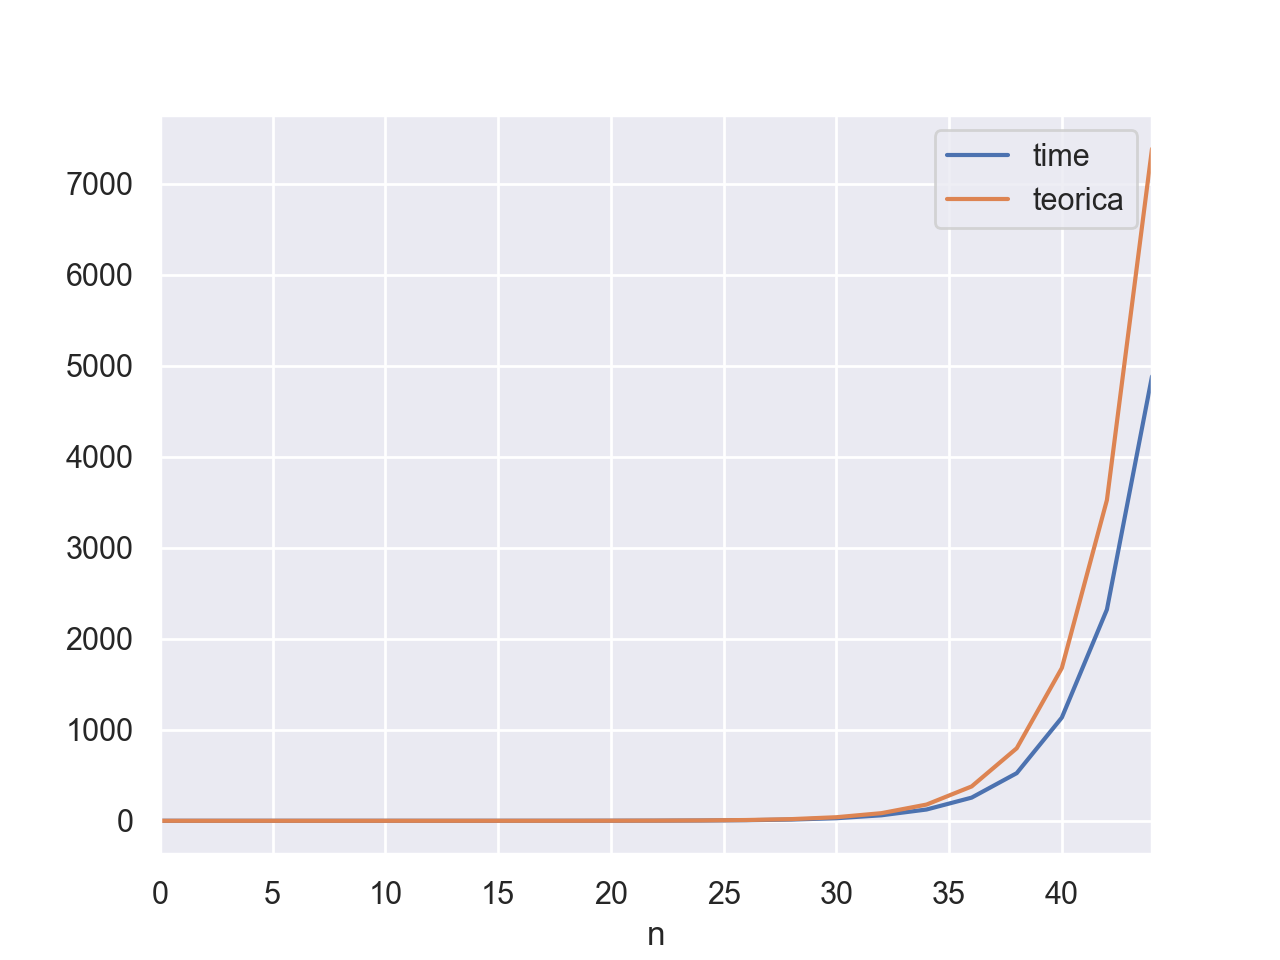
\includegraphics[width=1\linewidth]{img/Middle1}
     \caption{Comparación del gráfico de los resultados contra la cota teórica}
   \end{minipage}\hfill
   \begin{minipage}{0.6\textwidth}
     \centering
     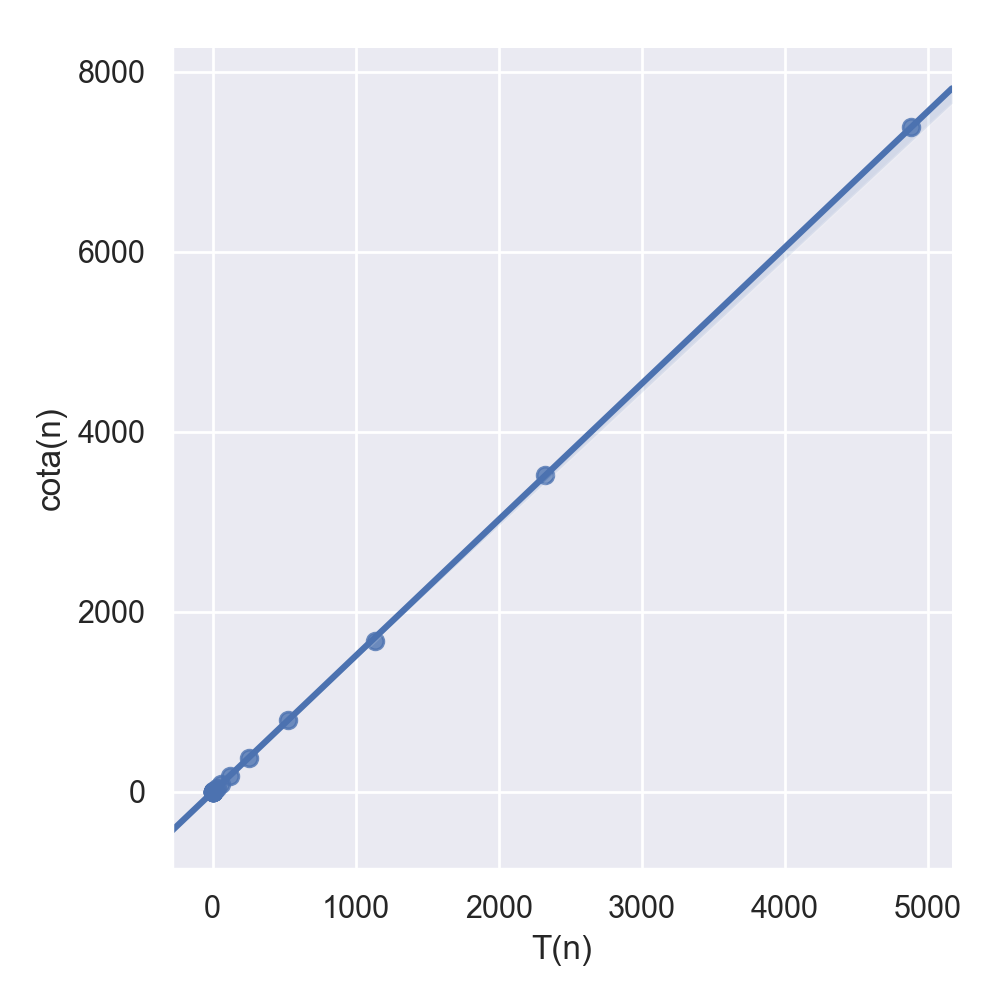
\includegraphics[width=1\linewidth]{img/Middle2}
     \caption{Correlación entre algoritmo y cota teórica}
   \end{minipage}
\end{figure}

Como podemos observar en el primer gráfico, parecería ser que el tiempo de ejecución se ajusta fuertemente a la cota teórica. Ambas funciones parecen tener un crecimiento similar, pero podemos corroborar esto más apropiadamente con el segundo gráfico. Aquí, vemos que nuestros datos tienen una correlación positiva casi perfecta con la cota teórica. La recta de cuadrados mínimos cubre casi perfectamente a nuestros datos.
\label{sec:experimentacion}
